\documentclass[../../main.tex]{subfiles}
\begin{document}
\graphicspath{{./figures}}
\chapter{Preprocesamiento de los datos adquiridos}\label{cap::preproc}
Las señales externas son muestreadas por el ADC a 65~MSps en un ancho de banda de 25~MHz como se desarrolló en el \cref{sec::planteo-front-end}. Sin embargo, los \textit{beams} de salida poseen un ancho de banda de apenas 25~kHz, de manera que puede reducirse considerablemente tanto el ancho de banda como la tasa de muestreo. Si se lograse centrar el ancho de banda de un  \textit{beam} en banda base por ejemplo, este solo ocuparía $12.5\un{kHz}$. Esto permitiría teóricamente reducir el ancho de banda de trabajo a $12.5\un{kHz}$ y trabajar con una tasa de muestreo ligeramente superior a 25~kSps cumpliendo con el teorema del muestreo. \cite{teorema-del-muestreo}.

Como se dijo en el \cref{sec::planteo-sist-adq}, esta parte del \textit{core} de adquisición se desarrolla en el presente proyecto. Su diseño, implementación y validación se realizaron primero de manera aislada e independiente a lo desarrollado en \cite{proyecto-jose} y, posteriormente, se integró dentro de dicho sistema.

\section{Requerimientos de diseño}
La etapa de preprocesamiento debe ser capaz de seleccionar uno o varios canales de frecuencia de 25~kHz de ancho de banda, a partir de ahora a estos se les llamará \textit{beams} o haces, reservándose el término \textit{canal} para los canales del ADC.

Luego, partiendo de la banda de UHF de 3~MHz de ancho de banda centrada en $18.5\un{MHz}$ tras el submuestreo, debe obtenerse a la salida uno o varios haces de 25~kHz de ancho de banda.

\section{Diseño conceptual}\label{sec::disenio-conceptual-preproc}
Se parte de la señal real ya submuestreada cuyo espectro está cetrado en $\pm 18.5\un{MHz}$ (ver figura \ref{fig::undersampling}) y su módulo  es simétrico respecto a la frecuencia $f = 0$, como se ilustra en la figura \ref{fig::espectro-inicial}. Dentro de cada triángulo en dicho gráfico se encuentran todos los haces de 25~kHz, replicados a ambos lados del espectro. Esto implica una redundancia de información que puede aprovecharse para optimizar la etapa de preprocesamiento.

Se propone entonces trabajar sobre solo una de estas réplicas mediante una mezcla compleja, esto es, una rotación del espectro \unsure{Agregar referencia?} que permita llevar una de las copias mostradas en \ref{fig::espectro-inicial} a banda base. En este caso es indistinto cuál de las copias se selecciona. 

Asumiendo RABG, se tiene en el espectro una densidad de potencia de ruido independiente de la frecuencia. \unsure{En realidad en el modelo la DEP es estrictamente constante, pero eso no es lo que muestro en las figuras}
Tras el corrimiento de una de las réplicas a BB se procede a realizar también un filtrado como se muestra en la figura \ref{fig::espectro-banda-corrida} reduciendo el ancho de banda de trabajo de manera de filtrar gran parte del ruido entrante. Esta es una primera etapa de ganancia de preprocesamiento, la cual se analizó en el \cref{sec::ganancias-por-preproc}. 

Como puede verse en la figura \ref{fig::espectro-banda-corrida} el ancho de banda del filtro debe ser ligeramente superior a $1.5\un{MHz}$ de manera de tolerar el corrimiento Doppler producido durante la pasada del satélite, el cual puede alcanzar corrimientos de hasta $\pm 10\un{kHz}$, como se desarrolla en el apéndice \ref{ap::doppler}.

Una vez aislada una copia de la banda de interés, resta seleccionar el \textit{beam} que quiere recibirse. Esto puede hacerse mediante un procedimiento similiar al recién aplicado. En este caso, la señal es compleja ya que no hay simetría en el módulo del espectro respecto a $f = 0$, es decir que no existe la redundancia de información que existía al hacer la primer mezcla. Esto implica que el sentido en el que se rota el espectro es relevante.

En la figura \ref{fig::espectro-canal} se muestra el módulo del espectro tras realizar una segunda mezcla compleja partiendo de lo mostrado en la figura \ref{fig::espectro-banda-corrida} para trasladar a BB al haz de interés. El rectángulo en línea de puntos que se muestra en dicha figura representa el filtrado que debe aplicarse tras la mezcla, el cual atenuará el resto de la banda junto con la parte de la potencia de ruido que cae por fuera de la banda de interés, obteniéndose así una segunda ganancia de preprocesamiento.

Nuevamente, si bien los haces tienen 25~kHz de ancho de banda, el filtrado debe contemplar un margen para tolerar el corrimiento Doppler (ver apéndice \ref{ap::doppler}).

\figura[0.8]{espectro-inicial}{Ilustración del módulo del espectro a la entrada de la etapa del preprocesamiento. Se tiene la banda de interés sobre un piso de RABG. Se ve que el espectro es simétrico respecto a la frecuencia $f = 0$ ya que se trata de una señal real.}

\figura[0.8]{espectro-banda-corrida}{Módulo del espectro de la banda de interés trasladada a banda base y filtrada.}

\figura[0.8]{espectro-canal}{Módulo del espectro de la banda de interés centrada en el haz de interés tras la segunda mezcla compleja. El rectángulo en línea punteada representa el filtrado que debe aplicarse psoteriormente para atenuar el resto de la banda y el ruido que cae por fuera del ancho de banda del haz de interés.}

\section{Implementación en software}
A modo de primera comprobación del diseño conceptual previo a su implementación en hardware, se hizo una implementación en software \unsure{JQ: no sé si me gusta 'implementación en SW'. Tal vez lo cambiaría por 'Prueba de concepto en SW'} de la etapa de preprocesamiento empleando Python. 
Esta se encuentra en \texttt{Simulaciones/preprocesamiento.ipynb}. 

Partiendo de la señal submuestreada a 65~MSps mostrada en la figura \ref{fig::submuestreo} se aplicó un DDC \cite{DDC}, cuyo diagrama de bloques se muestra en la figura \ref{fig::DDC}. 
Este incluye un NCO el cual genera una exponencial compleja para realizar la rotación de espectro en sentido horario a una frecuencia de $18.5\un{MHz}$, de manera de trasladar la banda de $[-20\un{MHz}, -17\un{MHz}]$ a $[-1.5\un{MHz}, 1.5\un{MHz}]$. 

Ya en banda base, el DDC contiene una etapa de filtrado pasabajos, cuya frecuencia de corte se configuró como $f_c = 1.5\un{MHz}$ de manera de capturar toda la banda de interés dentro de la banda de paso del filtro. El filtrado aplicado fue de tipo Butterworth \cite{Butterworth}, sin embargo, el tipo de filtro elegido no tiene mayor relevancia en la presente implementación\unsure{JQ: por qué?}. Los coeficientes del mismo se obtuvieron mediante la función \texttt{butter} \cite{butter} de la librería de SciPy \cite{scipy} y el filtrado propiamente dicho se realizó usando la función \texttt{lfilter} \cite{lfilter} también de la librería de SciPy. 

Por último, el DDC posee una etapa de decimación en la cual se reduce la tasa de muestreo. Para determinar el factor de decimación debe tenerse en cuenta que la tasa de Nyquist \cite{Nyquist-rate} es ahora de 3~MHz, lo cual implica que la tasa actual de muestreo de 65~MSps podría reducirse hasta en un factor $65/3 = 21.66$ aproximadamente. 
No obstante, para esta implementación se eligió un factor de decimación de 10, de manera que la tasa de muestras a la salida del DDC resulta $6.5\un{MSps}$. La salida de este primer DDC se muestra en la figura \ref{fig::DDC-band}.

Teniendo toda la banda de UHF ya en BB, se procede a seleccionar un haz o \textit{beam} como se muestra en la figura \ref{fig::espectro-canal}. 
Para esto se instancia un nuevo DDC, el cual realiza la mezcla compleja para trasladar el haz a banda base, ejecuta un filtrado del haz con una frecuencia de corte de $f_c = 12.5\un{kHz}$\footnote{Al tratarse de una implementación de prueba, no se tuvo en cuenta el corrimiento Doppler. 
De tenerse en cuenta, debería aumentarse la frecuencia de corte del filtro aproximadamente 10~kHz por encima de la actual.} y finalmente una decimación. 
Para esta última se empleo un factor \todo{Agregar factor}. La salida de este segundo DDC se muestra en la figura \ref{fig::DDC-beam}, donde se observa que pudo aislarse un haz de 25~kHz de ancho de banda de manera exitosa.

\figura[0.7]{DDC}{Diagrama de bloques de un \textit{Digital Down Converter} (DDC).}

\begin{figure}[H]
    \centering
    \subcaptionbox{Salida del primer DDC encargado de trasladar la banda de interés a BB, filtrar y luego decimar con un factor 10..\label{fig::DDC-band}}
    {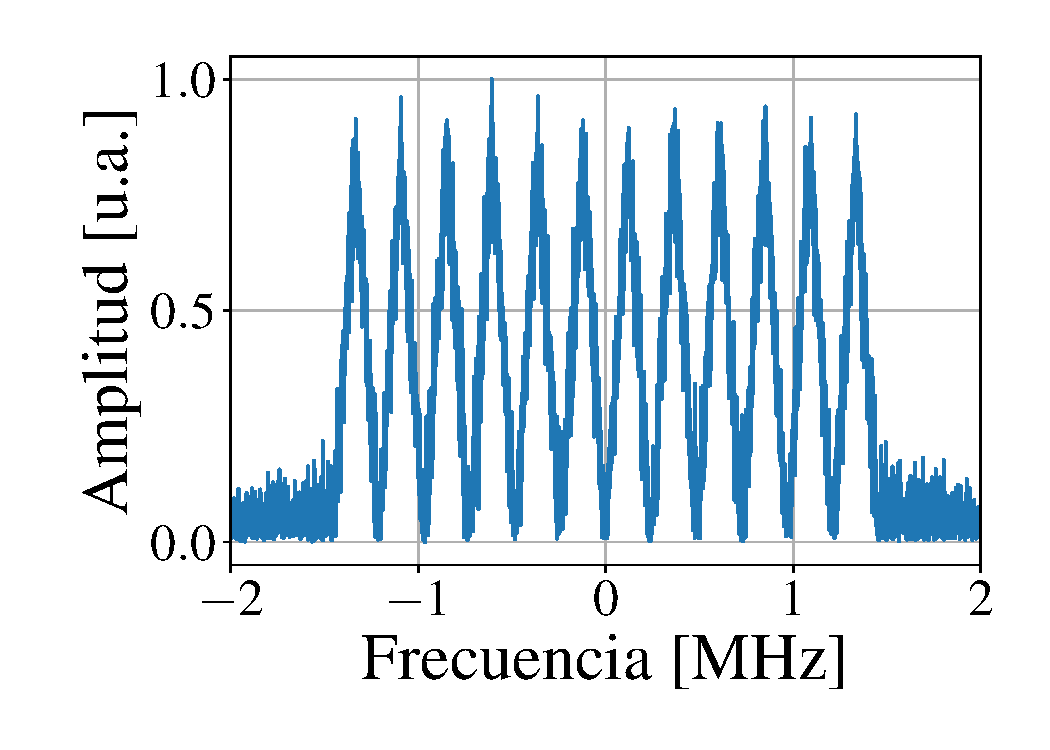
\includegraphics[width=0.49\linewidth]{DDC-band.pdf}}
    \hspace{\fill}%\\[1PC]
    \subcaptionbox{Salida del segundo DDC encargado de seleccionar un \textit{beam}, trasladarlo a BB, filtrarlo y reducir la tasa de muestreo. Se dibuja además una línea vertical en la frecuencia donde termina el canal de interés, esto es, $f = 12.5\un{kHz}$\label{fig::DDC-beam}}
    {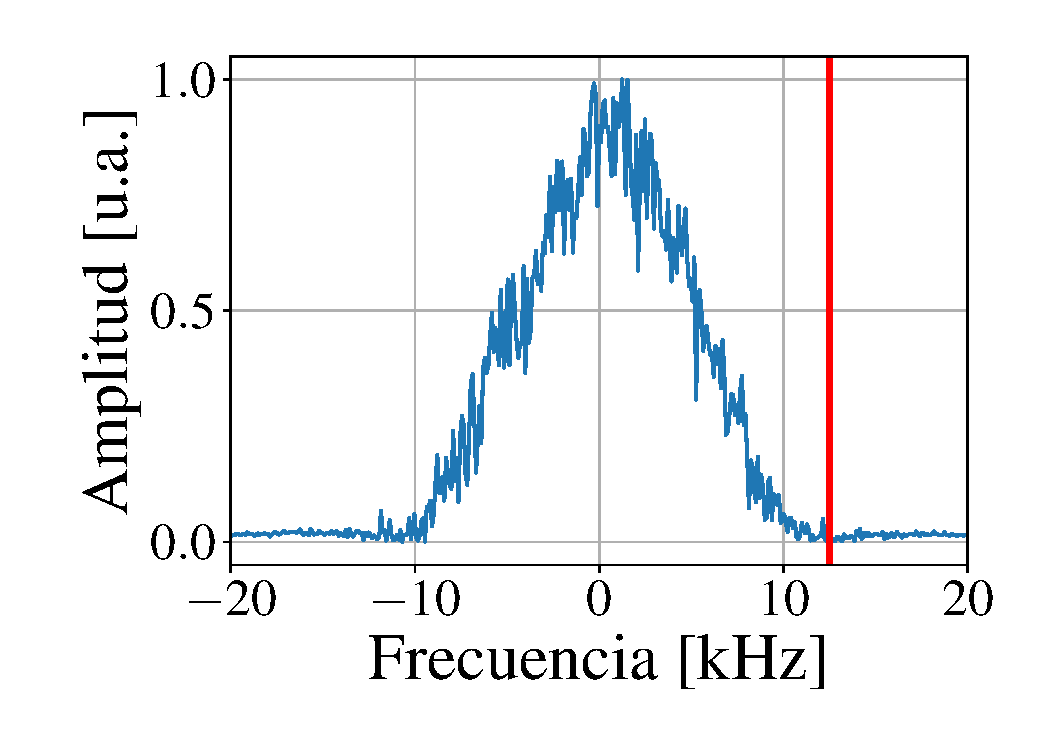
\includegraphics[width=0.49\linewidth]{DDC-beam.pdf}}
    \caption{Salida de las dos etapas de DDCs.}
    \label{fig::DDC-output}
\end{figure}

\section{Implementación en hardware}
%Uso clk de 260 MHz
Habiendo validado el diseño conceptual mediante una implementación en software se procede a realizar una implementación del mismo en la placa CIAA-ACC. Dado que el SoC Zynq-7030 incluido en la CIAA-ACC es fabricado por la compañía Xilinx, se hizo uso de su entorno de desarrollo, el cual incluye al software \textit{Vivado} \cite{vivado} para el desarrollo, síntesiss e implementación en la FPGA y al software \textit{Vitis Unified Software Platform} \cite{vitis} para el desarrollo y la compilación cruzada \cite{cross-compilation} del software para el PS. La versión del entorno de desarrollo usada en este proyecto fue la 2020.2.

La tasa de muestreo del AD9249 es de 65~MSps como se indica en la tabla \ref{tab::ADC}, esto fija la tasa de datos que tiene que procesar la FPGA y representa una frecuencia mínima de reloj a emplear. En base a esto, se eligió una frecuencia de reloj de 260~MHz para realizar el preprocesamiento de manera de disponer de 4 ciclos de reloj entre cada muestra que entrega el ADC\footnote{$260\un{MHz} = 4 \cdot 65\un{MHz}.$}. Esto puede otorgar cierta flexibilidad a la hora de diseñar el \textit{pipeline} de preprocesamiento.

\subsection{IPs empleadas}
\textit{Vivado} cuenta con interfaces o bloques propietarios en su librería de propiedad intelectual o IP \cite{IP-Xilinx}. Estos funcionan como caja negra para el usuario, recibiendo entradas y produciendo salidas acordes a su funcionalidad.

En el desarrollo de la etapa de preprocesamiento se utilizaron las IPs de \textit{Vivado} nombradas en la tabla \ref{tab::ip-vivado-preproc}.
\begin{table}[H]
    \centering
    \resizebox{\textwidth}{!}{%
    \begin{tabular}{|llc|}
    \hline
    \multicolumn{3}{|c|}{\textbf{IPs nativas utilizadas}}                                                                                                                                                                                                                                                        \\ \hline
    \multicolumn{1}{|l|}{\textbf{Nombre}}    & \multicolumn{1}{l|}{\textbf{Función}}                                                                                                                                                                                  & \textbf{Documentación}                   \\ \hline
    \multicolumn{1}{|l|}{AXI Interconnect}   & \multicolumn{1}{l|}{\begin{tabular}[c]{@{}l@{}}Conecta uno o más dispositivos maestros AXI mapeados\\ en memoria a uno o más dispositivos esclavos mapeados\\ en memoria.\end{tabular}}                                & \cite{axi-interconnect} \\ \hline
    \multicolumn{1}{|l|}{Complex Multiplier} & \multicolumn{1}{l|}{\begin{tabular}[c]{@{}l@{}}Implementa multiplicadores complejos optimizados, de\\ alto rendimiento y compatibles con AXI4-Stream basados\\ en opciones especificadas por el usuario.\end{tabular}} & \cite{complex-mult}     \\ \hline
    \multicolumn{1}{|l|}{DDS Compiler}       & \multicolumn{1}{l|}{Genera señales sinusoidales.}                                                                                                                                                                      & \cite{dds-compiler}     \\ \hline
    \multicolumn{1}{|l|}{FIR Compiler}       & \multicolumn{1}{l|}{Genera un filtro tipo FIR.}                                                                                                                                                                        & \cite{fir-compiler}     \\ \hline
    \end{tabular}%
    }
    \caption{IPs nativas utilizadas en el desarrollo de la etapa de preprocesamiento.}
    \label{tab::ip-vivado-preproc}
    \end{table}

\subsection{Módulos desarrollados}
Además de emplear IPs de \textit{Vivado}, se desarrollaron módulos en VHDL accesibles en el directorio \texttt{Fpga/prj/preprocessing\_stage/src}. Dichos módulos y su función se mencionan a continuación en la tabla \ref{tab::ip-fran}\todo{JQ: revisar si falta alguno (FIFO input data mux?)}.

La integración de estos módulos con las IPs de Xilinx serán más claras en breve cuando se explique la composición del sistema implementado.

\begin{table}[H]
    \resizebox{\textwidth}{!}{%
    \begin{tabular}{|ll|}
    \hline
    \multicolumn{2}{|c|}{\textbf{Módulos desarrollados}}                                                                                                                                                                                                                                                                                                                                                               \\ \hline
    \multicolumn{1}{|l|}{\textbf{Nombre}}                                                   & \textbf{Función}                                                                                                                                                                                                                                                                                                         \\ \hline
    \multicolumn{1}{|l|}{\begin{tabular}[c]{@{}l@{}}DDS Compiler\\ Controller\end{tabular}} & \begin{tabular}[c]{@{}l@{}}Opera con la interfaz AXI4-Stream. Su entrada es la salida de\\ un DDS Compiler. Mediante el pulso de tready del protocolo\\ AXI4-Stream controla la tasa a la cual el DDS Compiler \\ genera nuevos datos, convirtiendola en cualquier submúltiplo de\\ la frecuencia de reloj.\end{tabular} \\ \hline
    \multicolumn{1}{|l|}{\begin{tabular}[c]{@{}l@{}}Valid Data\\ Holder\end{tabular}}       & \begin{tabular}[c]{@{}l@{}}Opera con la interfaz AXI4-Stream. Sostiene el último dato\\ válido en la salida hasta que llega uno nuevo.\end{tabular}                                                                                                                                                                      \\ \hline
    \multicolumn{1}{|l|}{Basic Counter}                                                     & \begin{tabular}[c]{@{}l@{}}Contador de ancho ajustable que se incrementa cada N \\ ciclos de reloj, con N configurable.\end{tabular}                                                                                                                                                                                     \\ \hline
    \multicolumn{1}{|l|}{Zero Padder}                                                       & \begin{tabular}[c]{@{}l@{}}Convierte una señal de N bits en una de M bits con M\textgreater{}N\\ agregando ceros ya sea a derecha o a izquierda.\end{tabular}                                                                                                                                                            \\ \hline
    \multicolumn{1}{|l|}{Data Source Mux}                                                   & \begin{tabular}[c]{@{}l@{}}Multiplexor con 3 entradas tipo AXI4-Stream y una señal\\ de control.\end{tabular}                                                                                                                                                                                                            \\ \hline
    \multicolumn{1}{|l|}{AXI Slave Reg}                                                     & Bloque de registros que implementan el protocolo AXI4-Lite.                                                                                                                                                                                                                                                              \\ \hline
    \multicolumn{1}{|l|}{CDC Two FF Sync}                                                   & \begin{tabular}[c]{@{}l@{}}Dos FF en serie. Sirven para sincronizar un bit de una señal\\ asíncrona.\end{tabular}                                                                                                                                                                                                        \\ \hline
    \multicolumn{1}{|l|}{CDC Comparator}                                                    & Compara dos entradas y la asigna a la salida en caso de ser iguales.                                                                                                                                                                                                                                                     \\ \hline
    \end{tabular}%
    }
    \caption{Módulos desarrollados en VHDL para el desarrollo de la etapa de preprocesamiento.}
    \label{tab::ip-fran}
    \end{table}

\subsection{Filtros y decimación}
%Aritmética de punto fijo, ver bitácora
\todo{Evaluar bien los filtros}


\subsection{Herramientas de \textit{debug}}
En todo desarrollo resulta importante incorporar herramientas para poder \textit{debuggear} el sistema cuando algo no esté funcionando. Con este propósito se empleó el módulo \texttt{Data Source Mux} mencionado en la tabla \ref{tab::ip-fran} al cual se conectaron tres entradas:
\begin{itemize}
    \item Los datos del ADC. Este es el modo de operación normal, no de \textit{debug}.
    \item Una instancia del módulo \texttt{Basic Counter} (ver tabla \ref{tab::ip-fran}).
    \item Una instancia del IP DDS Compiler (ver tabla \ref{tab::ip-vivado-preproc}) generando un coseno a una frecuencia conocida.
\end{itemize}

El multiplexor se controla mediante un registro en el módulo \texttt{AXI Slave Reg} conectado a su vez al IP AXI Interconnect.

\subsection{Cruces de dominio de reloj (CDCs)}
Un dominio de reloj se compone de todos los elementos de un circuito lógico que operan bajo la misma señal de \textit{clock}.

Al realizar desarrollo en hardware, una situación que se presenta con regularidad es la necesidad de sincronizar con un dado reloj una señal que proviene de otro dominio de reloj. Esta situación recibe el nombre de \textit{Clock Domain Crossing} (CDC) y debe ser manejada de manera de poder asegurar el cumplimiento de los tiempos de \textit{setup} y \textit{hold} de los \textit{flip-flops} controlados por el nuevo reloj.

En el caso de la señal de control del \texttt{Data Source Mux}, la misma se encuentra dentro del dominio de reloj del AXI Interconnect (el cual generalmente viene dado por el PS). Al tratarse de una señal lenta ya que cambia en tiempos muy largos, puede sincronizarse en el nuevo dominio de reloj (esto es, el de 260~MHz) como si se tratara de una señal asíncrona. Para esto se hace uso del módulo \texttt{CDC Two FF Sync}.

Sin embargo, dicho módulo por si solo se emplea para sincronizar un único bit \todo{referencia?}. En este caso, la señal de control del multiplexor tiene 2 bits (hay 3 entradas), en consecuencia, para asegurar la integridad de la señal en el CDC se emplean dos \texttt{CDC Two FF Sync} en serie y se comparan sus salidas con el módulo \texttt{CDC Comparator} como se muestra en la figura \ref{fig::CDC-preproc}. Si ambas salidas son iguales, entonces la señal se sincroniza exitósamente al dominio de reloj de 260~MHz.

\figura{CDC-preproc}{Sincronizador de 2 bits para señales lentas empleado para realizar el CDC de la señal de control del multiplexor desde el dominio de reloj del AXI Interconnect al dominio de reloj de 260~MHz.}

\subsection{Implementación en \textit{Vivado}}
Interconectando los bloques de IP de las tablas \ref{tab::ip-vivado-preproc} y \ref{tab::ip-fran} puede implementarse el diseño conceptual descrito en la sección \ref{sec::disenio-conceptual-preproc}. Dicha interconexión se muestra en la figura \ref{fig::bd-preproc}, la cual corresponde al diagrama de bloques instanciado en \textit{Vivado}. 

\todo{Ampliar, explicar jerarquías, qué hacemos con el complex gain?}

\figura{bd-preproc}{BD preproc}

\section{Verificación con UVM}
Habiendo implementado el diseño en \textit{Vivado}, se procedió a verificar su correcto funcionamiento mediante simulaciones. \textit{Vivado} provee herramientas de simulación, sin embargo resultan demasiado lentas y demandantes en términos computacionales. Para lograr simulaciones más rápidas se hizo uso del simulador de la empresa Siemens \textit{Questa Advanced Simulator} \cite{questa}. \unsure{Mencionamos a Questa o mejor me ahorro esto??}

Para el desarrollo de la simulación se utilizó \textit{Universal Verification Methodology} (UVM) \cite{uvm}. Este comenzó como un una librería de clases para el desarrollo de simulaciones en \textit{SystemVerilog} creado por la empresa Accellera para proveer un estándar en el ámbito de la verificación. Finalmente, UVM fue adoptado como estándar por la IEEE \cite{uvm-ieee}.

El para las simulaciones se encuentra en el directorio \texttt{Fpga/prj/preprocessing\_stage/sim/}.

\subsection{Estructura de la simulación}
La simulación se desarrolló de acuerdo al estándar UVM, cuya estructura se muestra en la fiugra \ref{fig::uvm-structure}. Las funciones de cada uno de los componentes se detalla en la tabla \todo{ref}

\todo{hacer tabla con componentes y descripción}

La simulación se estructuró en cinco archivos principales, ubicados en \texttt{Fpga/prj/preprocessing\_stage/sim/tb/}, estos son:

\todo{Tabla con archivos y descripción}

Se emplearon además dos tipos de \texttt{UVM Agent}, uno para simular el comportamiento del ADC y otro para simular un agente que opera de acuerdo al protocolo \textit{AXI4-Lite}\cite{AXI-4}. \change{Expandir, escribir mejor}

\figura[0.7]{uvm-structure}{Estructura del estándar UVM \cite{uvm}.}

\subsection{Casos simulados y resultados}
%Un solo tono a 19.51 MHz
%Un solo tono con ruido
%Tres tonos sin y con ruido



\section{Integración con el sistema de adquisición}
\todo{JQ: hay un montón de técnicas de CDC que se usaron (sincronizadores de nivel, de pulso, vector quasiestático, vector con pulso de valid delayeado...). Mencionaría todas las técnicas utilizadas, y un ejemplo de algún punto de dónde se hayan usado}
\subsection{Recreación del proyecto preexistente}

\subsection{Adaptaciones necesarias}
%Clock a 260, CDCs
%División en varios bloques para minimizar replicas (16 canales)
%Aumento dato fifo (32 bits en lugar de 16)
%Uso de dos shorts como complex
%JQ: cambio a RTL top, corte de adc_receiver para poder usar única etapa de procesamiento, mejoras de timing...
\subsection{Otras modificaciones}
%constraints - false paths
%Uso de complemento a 2
%Raw data path para calibracion
%Cambio de índices
%Fifo input mux

\subsection{Refactorización del código preexistente}
%Simplificación del adc_receiver
%Eliminación del bd_top para poder instanciar bds
%Incorporación del data_handler
%Ordenamiento natural de los canales
\section{Ampliaciones}
%Mas herramientas de debug, todas las salidas del mux
\subsection{Incorporación de múltiples haces}
\subsection{Optimizaciones}
\end{document}